\documentclass[tikz, border=10pt]{standalone}

\usepackage{tikz}

\tikzset{
    % declare parabola and line equations
    declare function={
        f(\x) = (\x)^2 - 4*\x + 4;
        g(\x) = \x - 2.25;
    },
    % point style
    dot/.style = {fill, circle, inner sep=3pt},
    % secant line style
    dashed line/.style = {shorten >=-1.5cm, shorten <=-1.5cm, dash pattern=on4pt off2pt}
}

\begin{document}
    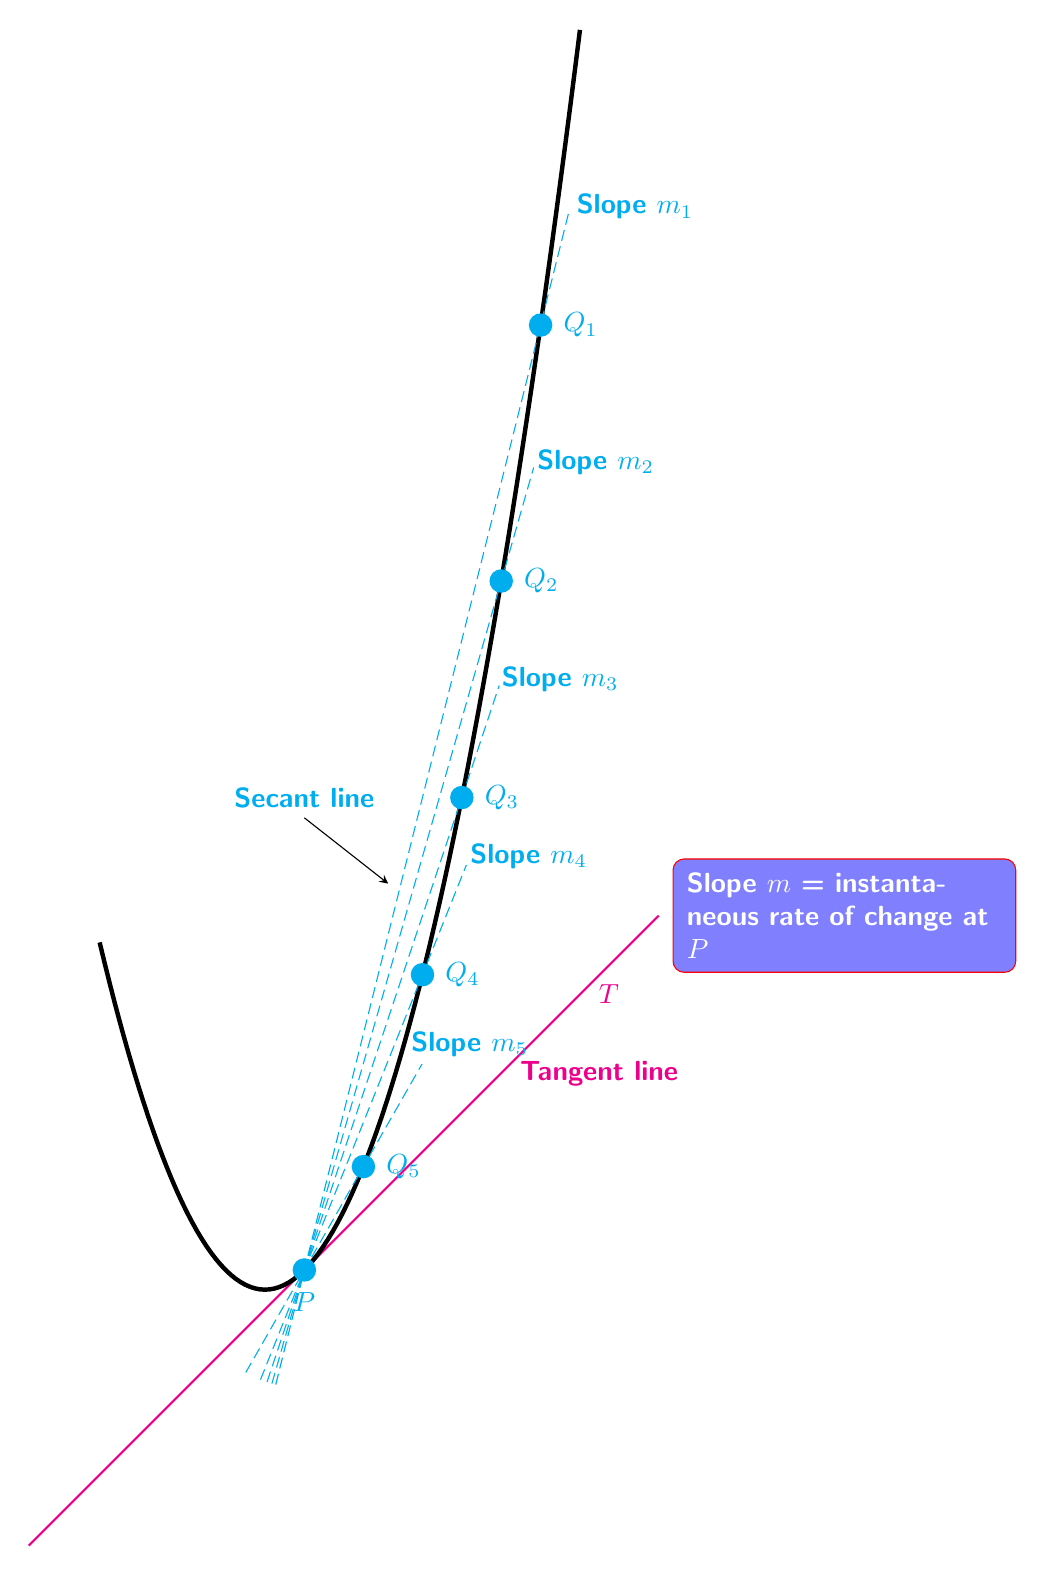
\begin{tikzpicture}
        \sffamily\bfseries
        % specify points on parabola
        \coordinate (P) at (2.5, {f(2.5)});
        \coordinate (Q5) at (3.25, {f(3.25)});
        \coordinate (Q4) at (4, {f(4)});
        \coordinate (Q3) at (4.5, {f(4.5});
        \coordinate (Q2) at (5, {f(5)});
        \coordinate (Q1) at (5.5, {f(5.5)});
        % draw tangent line
        \draw[thick, magenta] plot[smooth, domain=-1:7] (\x, {g(\x)});
        % draw parabola
        \draw[ultra thick] plot[samples=100, domain=-0.1:6] (\x, {f(\x)});
        % draw secant lines and label points
        \draw[cyan, dashed line] (P) node[dot, label={below:$P$}] {} -- (Q5) node[dot, label={right:$Q_5$}] {} node[shift={(1.35cm, 1.55cm)}] {Slope $m_5$};
        \draw[cyan, dashed line] (P) -- (Q4) node[dot, label={right:$Q_4$}] {} node[shift={(1.35cm, 1.5cm)}] {Slope $m_4$};
        \draw[cyan, dashed line] (P) -- (Q3) node[dot, label={right:$Q_3$}] {} node[shift={(1.25cm, 1.5cm)}] {Slope $m_3$};
        \draw[cyan, dashed line] (P) -- (Q2) node[dot, label={right:$Q_2$}] {} node[shift={(1.2cm, 1.5cm)}] {Slope $m_2$};
        \draw[cyan, dashed line] (P) -- (Q1) node[dot, label={right:$Q_1$}] {} node[shift={(1.2cm, 1.5cm)}] {Slope $m_1$} node[pos=0.4] (PQ1) {};

        \draw (5, {g(5)}) node[right=3pt, magenta] {Tangent line};
        \draw (6, {g(6)}) node[right=3pt, magenta] {$T$};
        \draw (7, {g(7)}) node[right=5pt, text width=4cm, fill=blue!50, text=white, rounded corners, inner sep=5pt, draw=red] {Slope $m$ = instantaneous rate of change at $P$};
        \draw (2.5, {f(4.5)}) node[cyan] (secant line) {Secant line};
        \draw[-stealth] (secant line.south) -- (PQ1);
    \end{tikzpicture}
\end{document}